\documentclass[12pt]{article}
\usepackage[utf8]{inputenc}
\usepackage[
a4paper,		% papel A4
left=2cm,		% margem esquerda
right=2cm,		% margem direita
top=2cm,		% margem superior
bottom=2cm		% margem inferior
]{geometry}
\usepackage[T1]{fontenc}	
\usepackage{array,latexsym}
\usepackage{amsmath,amsfonts,amssymb,amsthm,mathabx,amstext}
\usepackage{dsfont}	% Conjuntos: $\mathds{N, Z, Q, R, C}$
\usepackage{graphicx}
\begin{document}
\begin{center}
	Universidade Federal da Paraíba\\
	Probabilidade II\\
	Paulo Ricardo Seganfredo Campana 
\end{center}
\noindent Questão 1.\\

\noindent a)\\

$S_{X}=\{2,3,4,5,6,7,8,9,10,11,12\}$\\

\begin{tabular}{c|c|c|c|c|c|c|c|c|c|c|c}
	$X$ & 2 & 3 & 4 & 5 & 6 & 7 & 8 & 9 & 10 & 11 & 12 \\
	\hline
	$P(X=x)$ & $\dfrac{1}{36}$ & $\dfrac{2}{36}$ & $\dfrac{3}{36}$ & $\dfrac{4}{36}$ & $\dfrac{5}{36}$ & $\dfrac{6}{36}$ & $\dfrac{5}{36}$ & $\dfrac{4}{36}$ & $\dfrac{3}{36}$ & $\dfrac{2}{36}$ & $\dfrac{1}{36}$ \\	
\end{tabular}\\

\noindent b)\\

$S_{X}=\{1,2,3,4,5,6,8,9,10,12,15,16,18,20,24,25,30,36\}$\\

\noindent\begin{tabular}{c|c|c|c|c|c|c|c|c|c|c|c|c|c|c|c|c|c|c}
	$X$ & 1 & 2 & 3 & 4 & 5 & 6 & 8 & 9 & 10 & 12 & 15 & 16 & 18 & 20 & 24 & 25 & 30 & 36 \\
	\hline
	$P(X=x)$ & $\dfrac{1}{36}$ & $\dfrac{2}{36}$ & $\dfrac{2}{36}$ & $\dfrac{3}{36}$ & $\dfrac{2}{36}$ & $\dfrac{4}{36}$ & $\dfrac{2}{36}$ & $\dfrac{1}{36}$ & $\dfrac{2}{36}$ & $\dfrac{4}{36}$ & $\dfrac{2}{36}$ & $\dfrac{1}{36}$ & $\dfrac{2}{36}$ & $\dfrac{2}{36}$ & $\dfrac{2}{36}$ & $\dfrac{1}{36}$ & $\dfrac{2}{36}$ & $\dfrac{1}{36}$ \\	
\end{tabular}\\

\noindent Questão 2.\\

\noindent a)\\

$\displaystyle\sum_{x=0}^{\infty}c2^{-x}=1$\qquad\qquad
$\displaystyle\sum_{x=0}^{\infty}\left(\dfrac{1}{2}\right)^{x}=\dfrac{1}{c}$\qquad\qquad
$\dfrac{1}{1-\frac{1}{2}}=\dfrac{1}{c}$\qquad\qquad
$\dfrac{1}{2}=\dfrac{1}{c}$\qquad\qquad
$c=\dfrac{1}{2}$\\

\noindent b)\\

$P(X\leq2)=P(X=0)+P(X=1)+P(X=2)$\\

$\dfrac{1}{2}\left(2^{-0}+2^{-1}+2^{-2}\right)$\qquad\qquad
$\dfrac{1}{2}\left(1+\dfrac{1}{2}+\dfrac{1}{4}\right)\qquad\qquad$
$\dfrac{7}{8}$\\

\noindent c)\\

$P(X>5)=1-P(X\leq5)=P(X=0)+P(X=1)+P(X=2)+...+P(X=5)$\\

$1-\dfrac{1}{2}\left(2^{-0}+2^{-1}+2^{-2}+2^{-3}+2^{-4}+2^{-5}\right)$\\

$1-\dfrac{1}{2}\left(\dfrac{32}{32}+\dfrac{16}{32}+\dfrac{8}{32}+\dfrac{4}{32}+\dfrac{2}{32}+\dfrac{1}{32}\right)$\qquad\qquad
$1-\dfrac{63}{64}$\qquad\qquad
$\dfrac{1}{64}$\\

\noindent d)\\

$P(X\text{ ser ímpar})=P(X=2k+1)=\dfrac{1}{2}(2^{-1}+2^{-3}+2^{-5}...)$\\

$\dfrac{1}{2}\displaystyle\sum_{k=0}^{\infty}\left(\dfrac{1}{2}\right)^{2k+1}$\qquad\qquad
$\displaystyle\dfrac{1}{4}\sum_{k=0}^{\infty}\left(\dfrac{1}{2}\right)^{2k}$\qquad\qquad
$\displaystyle\dfrac{1}{4}\sum_{k=0}^{\infty}\left(\dfrac{1}{4}\right)^k$\qquad\qquad
$\dfrac{1}{4}\cdot\dfrac{1}{1-\frac{1}{4}}$\qquad\qquad
$\dfrac{1}{3}$\\

\noindent Questão 3.\\

$F_{X}(x)=\displaystyle\int_{-\infty}^{x}2t^{-3}\mathds{I}_{(1,\infty)}(x)dt$\qquad\qquad
$\displaystyle\int_{1}^{x}2t^{-3}dt$\qquad\qquad
$-t^{-2}\biggr|_{1}^{x}$\qquad\qquad
$(-x^{-2}+1)\mathds{I}_{(1,\infty)}(x)$\\

$\displaystyle\int_{0.5}^{2}2x^{-3}\mathds{I}_{(1,\infty)}(x)dx$\qquad\qquad
$\displaystyle\int_{1}^{2}2x^{-3}dx$\qquad\qquad
$-x^{-2}\biggr|_{1}^{2}$\qquad\qquad
$-\dfrac{1}{4}+1$\qquad\qquad
$\dfrac{3}{4}$\\

\noindent Questão 4.\\

\noindent a)\\

$\displaystyle\int_{0}^{0.5}cxdx+\int_{0.5}^{1}c-cxdx=1$\qquad\qquad
$\dfrac{cx^{2}}{2}\biggr|_{0}^{0.5}+c\left(x-\dfrac{x^{2}}{2}\right)\biggr|_{0.5}^{1}=1$\\

$\dfrac{c}{8}+c\left(\dfrac{1}{2}-\dfrac{3}{8}\right)=1$\qquad\qquad
$\dfrac{c}{8}+\dfrac{c}{8}=1$\qquad\qquad
$\dfrac{c}{4}=1$\qquad\qquad
$c=4$\\

\noindent b)\\

\begin{figure}[h!]
	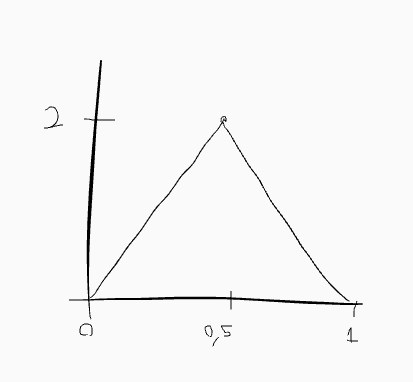
\includegraphics[scale=0.5]{4b}
\end{figure}

\noindent c)\\

$\displaystyle 4\int_{0.8}^{1}1-xdx$\qquad\qquad
$4\left(x-\dfrac{x^{2}}{2}\right)$\qquad\qquad
$4(0.5-0.8+0.32)$\qquad\qquad
$4(0.02)$\qquad\qquad
$0.08$\\

\noindent Para $P(0.25<x<0.75)$, percebe-se que é um intervalo simétrico em uma função simétrica em torno de $x=0.5$, portanto basta calcular $2P(0.25<x<0.5)$.\\

$\displaystyle 2\cdot4\int_{0.25}^{0.5}xdx$\qquad\qquad
$8\dfrac{x^{2}}{2}\biggr|_{0.25}^{0.5}$\qquad\qquad
$1-\dfrac{1}{4}$\qquad\qquad
$\dfrac{3}{4}$\\

\noindent Questão 5.\\

\noindent a)\\

$\displaystyle\int_{\mathds{R}}cx^{2}\mathds{I}_{(-1,1)}(x)dx=1$\qquad\qquad
$\displaystyle\int_{-1}^{1}cx^{2}dx=1$\qquad\qquad
$c\dfrac{x^{3}}{3}\biggr|_{-1}^{1}=1$\quad\quad
$\dfrac{c}{3}+\dfrac{c}{3}=1$\quad\quad
$c=\dfrac{3}{2}$\\

\noindent b)\\

$P\left(|X|>\dfrac{1}{2}\right)=P\left(X<-\dfrac{1}{2}\right)+P\left(X>\dfrac{1}{2}\right)$\\

$\displaystyle\int_{-1}^{-0.5}\dfrac{3}{2}x^{2}dx+\int_{0.5}^{1}\dfrac{3}{2}x^{2}dx$\qquad\qquad
$\dfrac{x^3}{2}\biggr|_{-1}^{-0.5}+\dfrac{x^3}{2}\biggr|_{0.5}^{1}$\\

$\left(-\dfrac{1}{16}+\dfrac{1}{2}\right)+\left(\dfrac{1}{2}-\dfrac{1}{16}\right)$\qquad\qquad
$\dfrac{7}{16}+\dfrac{7}{16}$\qquad\qquad
$\dfrac{7}{8}$\\

\noindent Questão 6.\\

\noindent a)\\

$\displaystyle\int_{\mathds{R}}\lambda e^{-\lambda x}\mathds{I}_{(0,\infty)}(x)dx=1$\qquad\qquad
$\lambda\displaystyle\int_{0}^{\infty}e^{-\lambda x}dx=1$\\

$\lambda\left(\dfrac{-e^{-\lambda x}}{\lambda}\right)\biggr|_{0}^{\infty}=1$\qquad\qquad 
$\lambda\left(0+\dfrac{1}{\lambda}\right)=1$\qquad\quad
$1=1$\qquad\qquad
é função densidade se $\lambda>0$\\

\noindent b)\\

$F_{X}(x)=\displaystyle\int_{-\infty}^{x}\lambda e^{-\lambda t}\mathds{I}_{(0,\infty)}dt$\qquad\qquad
$\lambda\displaystyle\int_{0}^{x}e^{-\lambda t}dt$\\

$\lambda\left(\dfrac{-e^{-\lambda t}}{\lambda}\right)\biggr|_{0}^{x}$\qquad\qquad
$-e^{-\lambda t}\biggr|_{0}^{x}$\qquad\qquad
$-e^{-\lambda x}+e^{0}$\qquad\qquad
$1-e^{-\lambda x}$\\

\noindent c)\\

$P(X\geq6)=1-P(X<6)$\\

$1-(1-e^{-6\lambda})$\qquad\qquad
$e^{-6\lambda}$\\

\noindent Questão 7.\\

\noindent a)\\

$\Gamma(\alpha+1)=\displaystyle\int_{0}^{\infty}t^{\alpha}e^{-t}dt$\qquad\qquad
$\left\{\begin{array}{@{}l@{}}
	u=t^{\alpha}\quad\Longrightarrow du=\alpha t^{\alpha-1}dt\\
	v=-e^{-t}\Longrightarrow dv=e^{-t}dt
\end{array}\right.$\\

$(-e^{-t}t^{\alpha})\biggr|_{0}^{\infty}+\alpha\displaystyle\int_{0}^{\infty}t^{\alpha-1}e^{-t}$\qquad\qquad
$\alpha\Gamma(\alpha)$\\

\noindent b)\\

$\Gamma(1)=\displaystyle\int_{0}^{\infty}t^{1-1}e^{-t}dt$\qquad\qquad
$\displaystyle\int_{0}^{\infty}e^{-t}dt$\qquad\qquad
$-e^{-t}\biggr|_{0}^{\infty}$\qquad\qquad
$0+1$\qquad\qquad
$\Gamma(1)=1$\\

\noindent c)\\

$\Gamma(n+1)=n\Gamma(n)$\\

$\Gamma(n+1)=n(n-1)\Gamma(n-1)$\\

$\Gamma(n+1)=n(n-1)(n-2)\Gamma(n-2)$\\

$\Gamma(n+1)= ...$\\

$\Gamma(n+1)=n(n-1)(n-2)\cdot...\cdot2\cdot1$\\

$\Gamma(n+1)=n!$\\

\noindent d)\\

$\Gamma\left(\frac{1}{2}\right)=\displaystyle\int_{0}^{\infty}t^{-\frac{1}{2}}e^{-t}dt\qquad\qquad\qquad\qquad t=u^{2}/2\qquad dt=udu$\\

$\displaystyle\int_{0}^{\infty}\left(\dfrac{u^{2}}{2}\right)^{-\frac{1}{2}}e^{-\frac{u^2}{2}} udu$\qquad\qquad
$\sqrt{2}\displaystyle\int_{0}^{\infty}u^{-1}e^{-\frac{u^2}{2}}udu$\qquad\qquad
$\sqrt{2}\displaystyle\int_{0}^{\infty}e^{-\frac{u^2}{2}}du$\\

$\Phi(x)=\displaystyle\int_{-\infty}^{x}\dfrac{1}{\sqrt{2\pi}}e^{-\frac{t^2}{2}}dt$\qquad\qquad
$\Phi(\infty)=\displaystyle\int_{-\infty}^{\infty}\dfrac{1}{\sqrt{2\pi}}e^{-\frac{t^2}{2}}dt=1$\qquad\qquad
$\displaystyle\int_{0}^{\infty}\dfrac{1}{\sqrt{2\pi}}e^{-\frac{t^2}{2}}dt=\dfrac{1}{2}$\\

$\sqrt{2}\sqrt{2\pi}\displaystyle\int_{0}^{\infty}\dfrac{1}{\sqrt{2\pi}}e^{-\frac{u^2}{2}}du$\qquad\qquad
$2\sqrt{\pi}\cdot \dfrac{1}{2}$\qquad\qquad
$\sqrt{\pi}$\\

\noindent Questão 8.\\

$\displaystyle\int_{-\infty}^{\infty}\dfrac{\beta^{\alpha}}{\Gamma(\alpha)}x^{\alpha -1}e^{-\beta x}\mathds{I}_{(0,\infty)}(x)dx=1$\\

$\dfrac{\beta^{\alpha}}{\Gamma(\alpha)}\displaystyle\int_{0}^{\infty}x^{\alpha -1}e^{-\beta x}dx=1\qquad\qquad\qquad\qquad t=\beta x\qquad dt=\beta dx$\\

$\dfrac{\beta^{\alpha}}{\Gamma(\alpha)}\displaystyle\int_{0}^{\infty}\left(\dfrac{t}{\beta}\right)^{\alpha -1}e^{-t}\dfrac{1}{\beta}dt=1$\\

$\dfrac{\beta^{\alpha}}{\Gamma(\alpha)}\dfrac{1}{\beta}\dfrac{1}{\beta^{\alpha -1}}\displaystyle\int_{0}^{\infty}t^{\alpha -1}e^{-t}dt=1$\\

$\dfrac{1}{\Gamma(\alpha)}\Gamma(\alpha)=1$\\

$1=1$\\

\end{document}